%% SW arkitektur: Logical View

Logical view skal danne et overblik over hvilke software pakker der befinder sig på vores platforme. Blokkene inde i de respektive pakker kan sammen med domænemodellen hjælpe med at give et overblik over hvilke klasser og kernemoduler der skal bruges.

\begin{figure}[htbp] \centering
{\includegraphics[scale=0.7]{filer/systemarkitektur/logical_view_devkit}}
\caption{Logical view for devkittet illustrer hvilke software pakker der befinder sig på Masteren }
\label{fig:Logical View Devkit8000}
\end{figure}

Figur \ref{fig:Logical View Devkit8000} illustrere hvilke software pakker der ligger på Masteren. Der er 3 pakker software da der arbejdes på en linux platform. I bunden har vi device driveren som skal håndtere SPI kommunikationen imellem devkit og PSoC. I midten ligger der en hardware API som håndtere hvordan informationen fra device driveren bliver sendt videre til applications pakken. Applications pakken tager sig af alt bruger UI samt log og fejlhåndtering.

\clearpage

%\textit{Applications} pakken består af alt den software som har med brugeren at gøre, dvs. UI og tilhørende controllers. Applications pakken tager imod input fra brugeren og reagerer på det enten ved at kalde nogle af sine egne controllers eller sende kommandoer til hardware APIen. Desuden får pakken data fra nedenstående pakker til at fremstå overskueligt over for brugeren.
%
%\clearpage
%
%\textit{Hardware API} pakken består af almindelige klasser som gør brug af file systemets kommandoer som f.eks open og close.
%
%\textit{Device Driver} pakken består af den software som håndtere alt hardware input og output. Hardware proxys inklusiv. 
\newenvironment{figure1}[1][]{\begin{figure}[#1]\vspace{3.0cm}}{\vspace{1.0cm}\end{figure}}
\begin{figure1}[htbp] \centering
{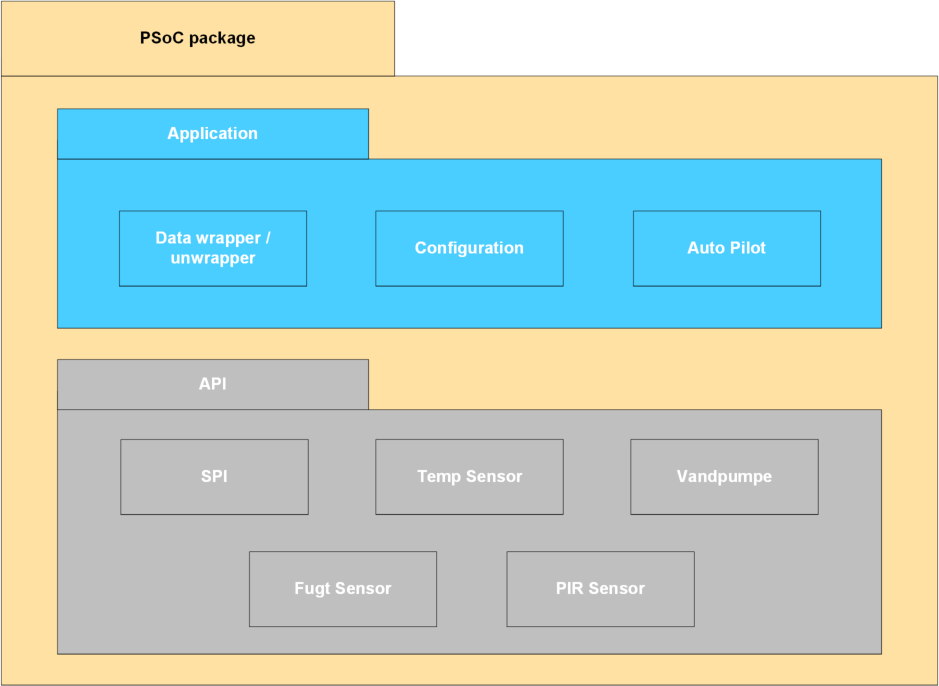
\includegraphics[scale=0.7]{filer/systemarkitektur/logical_view_psoc}}
\caption{Logical view for PSoC illustrer hvilke software pakker der befinder sig på enhederne}
\label{fig:Logical View PSoC}
\end{figure1}

Figur \ref{fig:Logical View PSoC} illustrere hvilke software pakker der ligger på enhederne. API pakken består af den software som håndterer hardwaren, dvs. den tager imod input og får formateret det til noget læseligt til applications pakken. Derudover står den for at få sendt de informationer applications pakken beder om på en effektiv og sikker måde. Applications pakken håndterer den indsamlede data som den får fra sensorene igennem API pakken. Denne data sammensættes ifølge protokollen og sendes til API pakken som får det sendt til devkittet. Pakken skal også håndtere data fra devkittet til at konfigurere de parametre der styre automatiseringen af vandingen som applications pakken også håndterer.

